\documentclass[xcolor=dvipsnames]{beamer}
\usepackage{amsmath}
\usepackage{relsize}
\usetheme{EastLansing} 
% Remove navigation bar
\setbeamertemplate{navigation symbols}{}
%%%%%% Design changes
\setbeamercolor{title}{fg=black, bg=green!50!blue!30!white}
\setbeamercolor{frametitle}{fg=black}
%
\setbeamercolor{block title}{fg=black, bg=green!50!blue!50!white}
\setbeamercolor{block body}{fg=black, bg=green!50!blue!30!white}
%
\setbeamercolor{block title alerted}{fg=black, bg=green!45!blue!50!white}
\setbeamercolor{block body alerted}{fg=black, bg=green!40!blue!30!white}
%
\setbeamercolor{block title example}{fg=black, bg=green!35!blue!50!white}
\setbeamercolor{block body example}{fg=black, bg=green!30!blue!30!white}
%
\setbeamercolor{palette primary}{fg=black, bg=green!50!blue!20!white}
\setbeamercolor{palette secondary}{fg=black, bg=green!60!blue!30!white}
\setbeamercolor{palette tertiary}{fg=black, bg=green!60!blue!40!white}
\setbeamercolor{palette quaternary}{fg=black, bg=green!30!blue!20!white}
%
\useinnertheme{circles}
\setbeamercolor{itemize item}{fg=black}
\setbeamercolor{itemize subitem}{fg=black}
\setbeamercolor{itemize subsubitem}{fg=black}
%
%%%%% Design changes %%%%%


% Tikz package
\usepackage{tikz}
\usetikzlibrary{positioning}
% General info
\title{Fachprojekt - Digital Entertainment Technologies}
\subtitle{WiSe 2021/2022 \\ TU Dortmund}
\author{E. Almsouti, C. Kolbe,  L. Labbert, A. Montag}
\institute{}
\date{01.02.2022}


%%%%%%%%%%%%%%%%%%%%%%%%%%%%%%%%%%%%%%%%%%%%%%%%%%%%%%%%%%%%%%%%%%%%%%
\begin{document}
%%%%%%%%%%%%%%%%%% Slide %%%%%%%%%%%%%%%%%%
\begin{frame}
\titlepage
\end{frame}

%%%%%%%%%%%%%%%%%% Slide %%%%%%%%%%%%%%%%%%
\begin{frame}{TuttiFrutti - Spielidee}
\begin{itemize}
\item Multiplayer Spiel
\item Einfach und schnelle Runden mit unterschiedlichen Leveln/Modi \item Vor allem für Freunde-Gruppen gedacht als "party game"
\item Free-for-all 
\end{itemize}

\end{frame}

%%%%%%%%%%%%%%%%%% Slide %%%%%%%%%%%%%%%%%%
\begin{frame}{TuttiFrutti - Infos}
\begin{itemize}
\item  Multiplayer via IP oder Steam (keine eigene Game-SteamID) 
\item 3rd Person
\item Keine hohen Performance-Anforderungen 
\item Ein Spiel besteht aus 4 Runden zwischen 90-150s 
\item Kein finales Ausscheiden aus einer Lobby möglich
\item Punkte werden auf die Spieler-Anzahl normiert

\end{itemize}

\end{frame}

%%%%%%%%%%%%%%%%%% Slide %%%%%%%%%%%%%%%%%%
\begin{frame}{TuttiFrutti - Schwerpunkte}
\begin{itemize}
	\item Multiplayer
	\begin{itemize}
		\item IP-basiert über kcp 
		\item Online über Steam
	\end{itemize}
	\item Presentation
	\begin{itemize}
		\item Eigener Player character 
		\item Player-Animations
		\item Particle effects
		\item Animiertes Menu 
		\item Player Konfiguration
	\end{itemize}
\end{itemize}

\end{frame}

%%%%%%%%%%%%%%%%%% Slide %%%%%%%%%%%%%%%%%%
\begin{frame}{Level - HillKing}
\begin{columns}
\begin{column}{0.5\textwidth}
	\begin{itemize}
		\item Aktive Platform wechselt alle 30" zufällig 
		\item Wenn man auf der Plattform steht bekommt man Punkte -$>$ andere Spieler durch Schubsen an Punkten hindern 
	\end{itemize}
\end{column}
\begin{column}{0.5\textwidth} 
	\begin{center}
		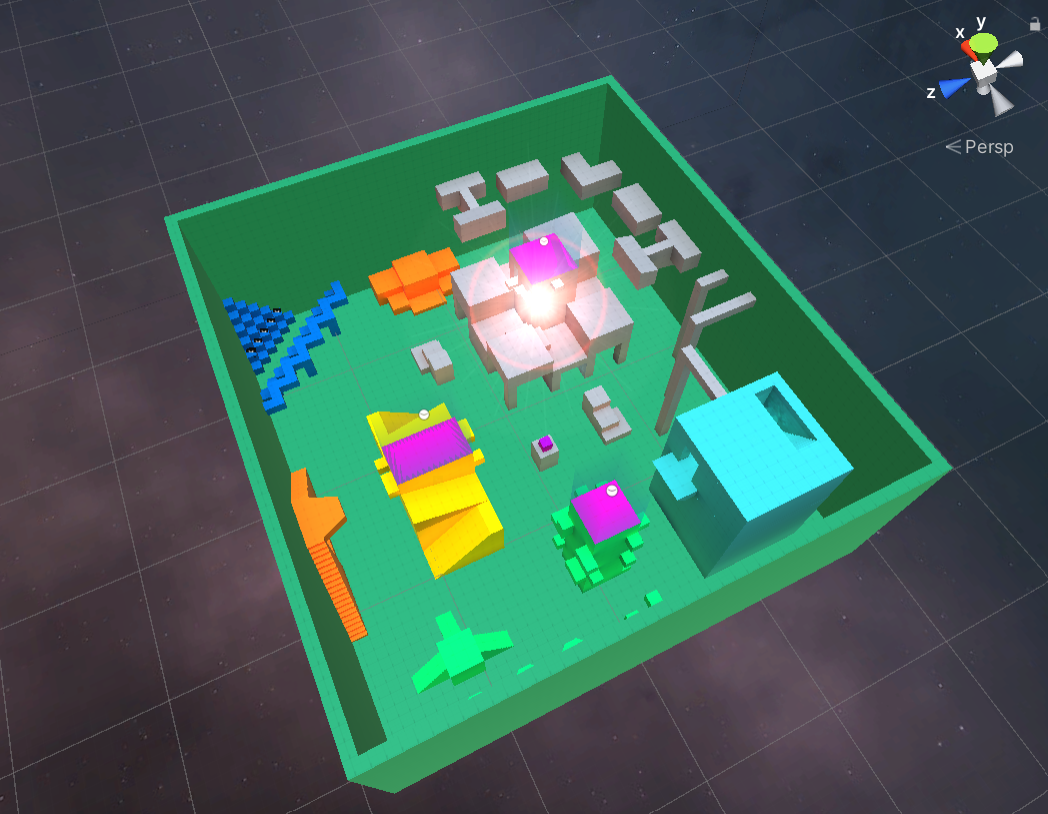
\includegraphics[width=0.9\textwidth]{level_hillking.png}
	\end{center}
\end{column}
\end{columns}

\end{frame}

%%%%%%%%%%%%%%%%%% Slide %%%%%%%%%%%%%%%%%%
\begin{frame}{Level - Crown}
\begin{columns}
\begin{column}{0.5\textwidth}
	\begin{itemize}
		\item Abhängig von der Spieler-Anzahl werden einzelne Spieler mit Kronen gespawnt 
		\item Man bekommt Punkte wenn man eine Krone hat -$>$ Kronen stehlen
	\end{itemize}
\end{column}
\begin{column}{0.5\textwidth} 
	\begin{center}
		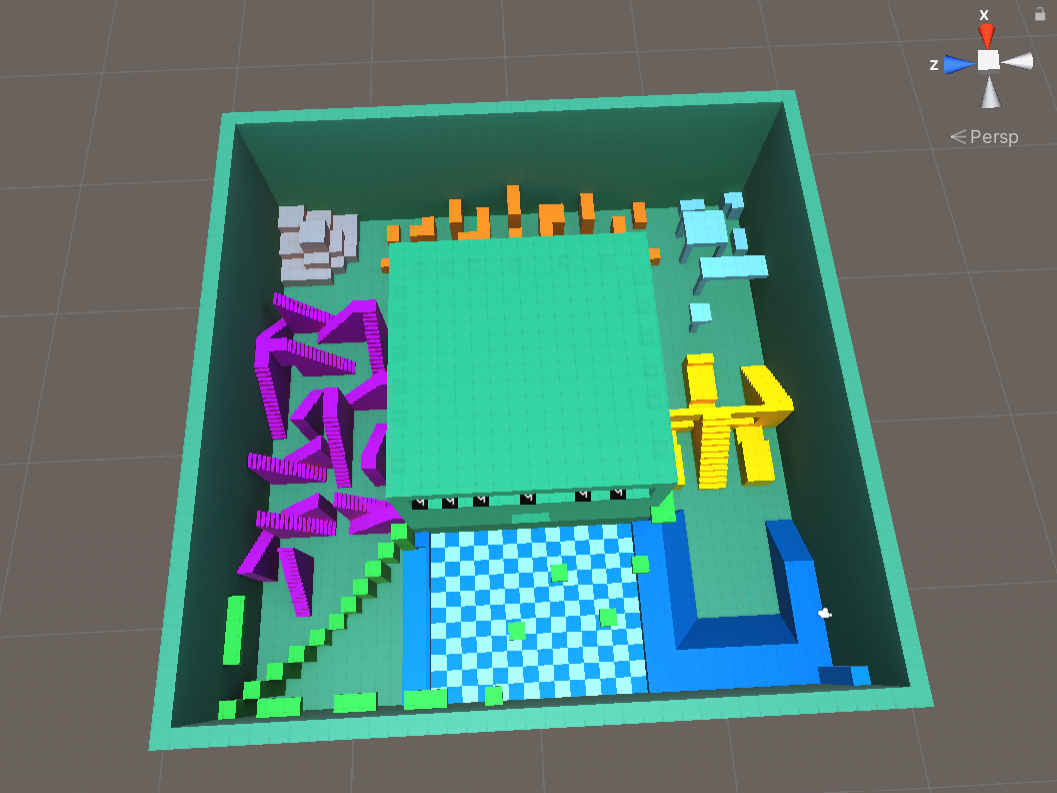
\includegraphics[width=0.9\textwidth]{level_crown.png}
	\end{center}
\end{column}
\end{columns}

\end{frame}

%%%%%%%%%%%%%%%%%% Slide %%%%%%%%%%%%%%%%%%
\begin{frame}{Level - RunTheLine}
\begin{columns}
\begin{column}{0.5\textwidth}
	\begin{itemize}
		\item Rennen zum Ziel!
		\item Der Spieler muss mehreren Hindernissen ausweichen und als erstes ins Ziel kommen.
		\item Die Punkte werden abhängig von der Positionierung des Spielers verteilt.
	\end{itemize}
\end{column}
\begin{column}{0.5\textwidth} 
	\begin{center}
		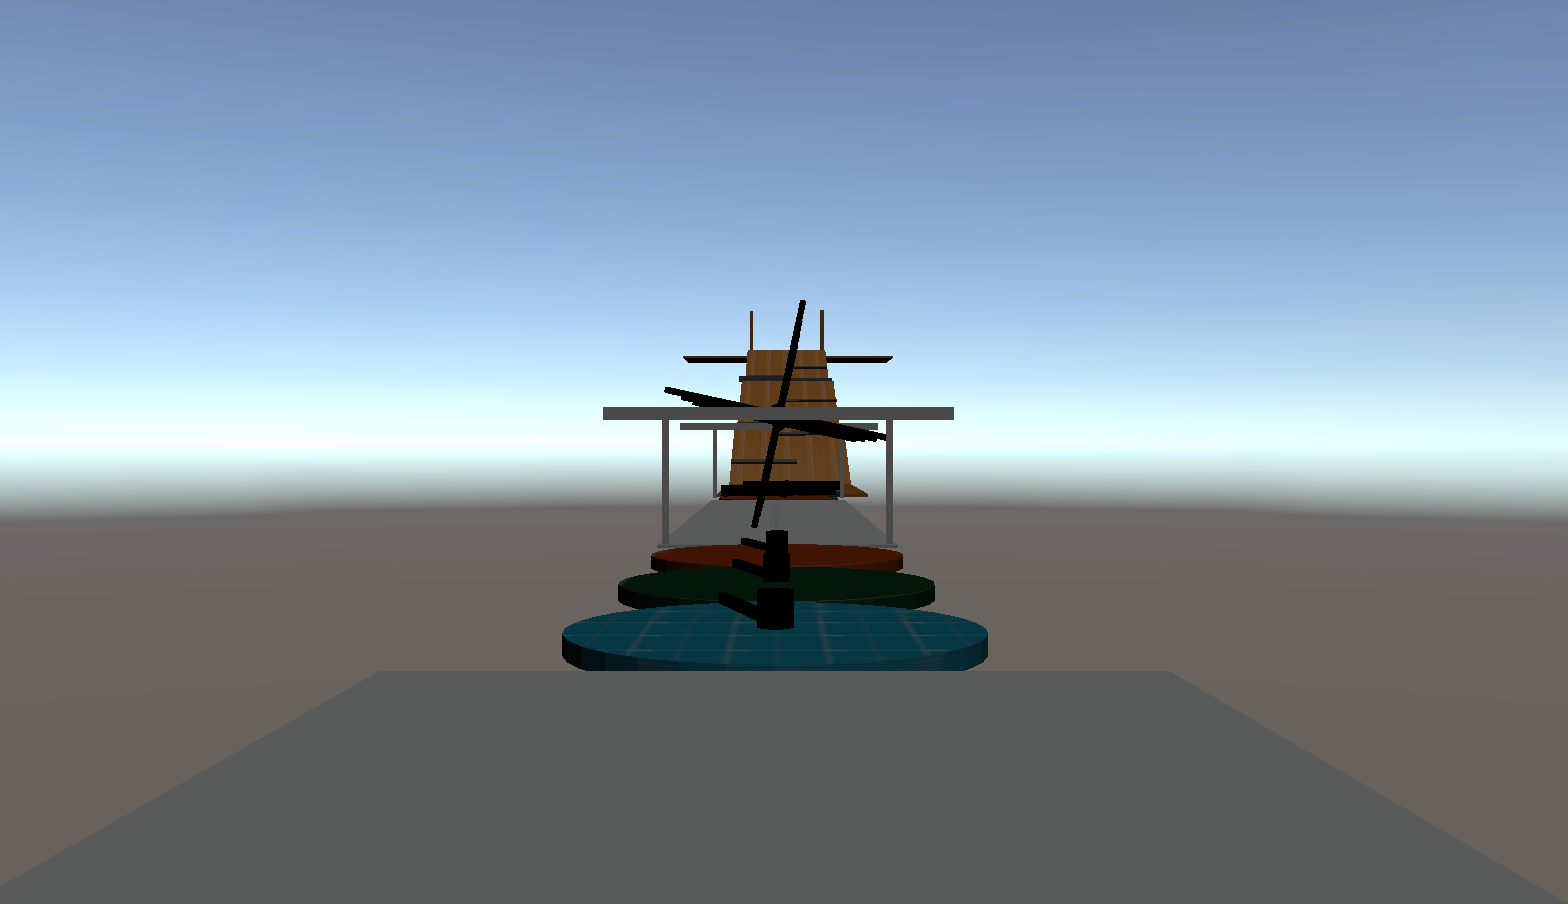
\includegraphics[width=0.9\textwidth]{runthelinpic.png}
	\end{center}
\end{column}
\end{columns}

\end{frame}

%%%%%%%%%%%%%%%%%% Slide %%%%%%%%%%%%%%%%%%
\begin{frame}{Level - PerfectMatch}
\begin{columns}
\begin{column}{0.5\textwidth}
	\begin{itemize}
		\item Halte alle drei Runden durch!
		\item Spielfeld: 16 Plattformen, die zu einem 4x4 Raster aufgebaut sind.
		\item Der Spieler muss sich, die auf den Plattformen angezeigten, Früchte merken und sich auf die richtige Plattform stellen wenn die Eliminierung stattfindet.
		\item Punkte werden anhand der durchgehaltenen Runden verteilt.
	\end{itemize}
\end{column}
\begin{column}{0.5\textwidth} 
	\begin{center}
		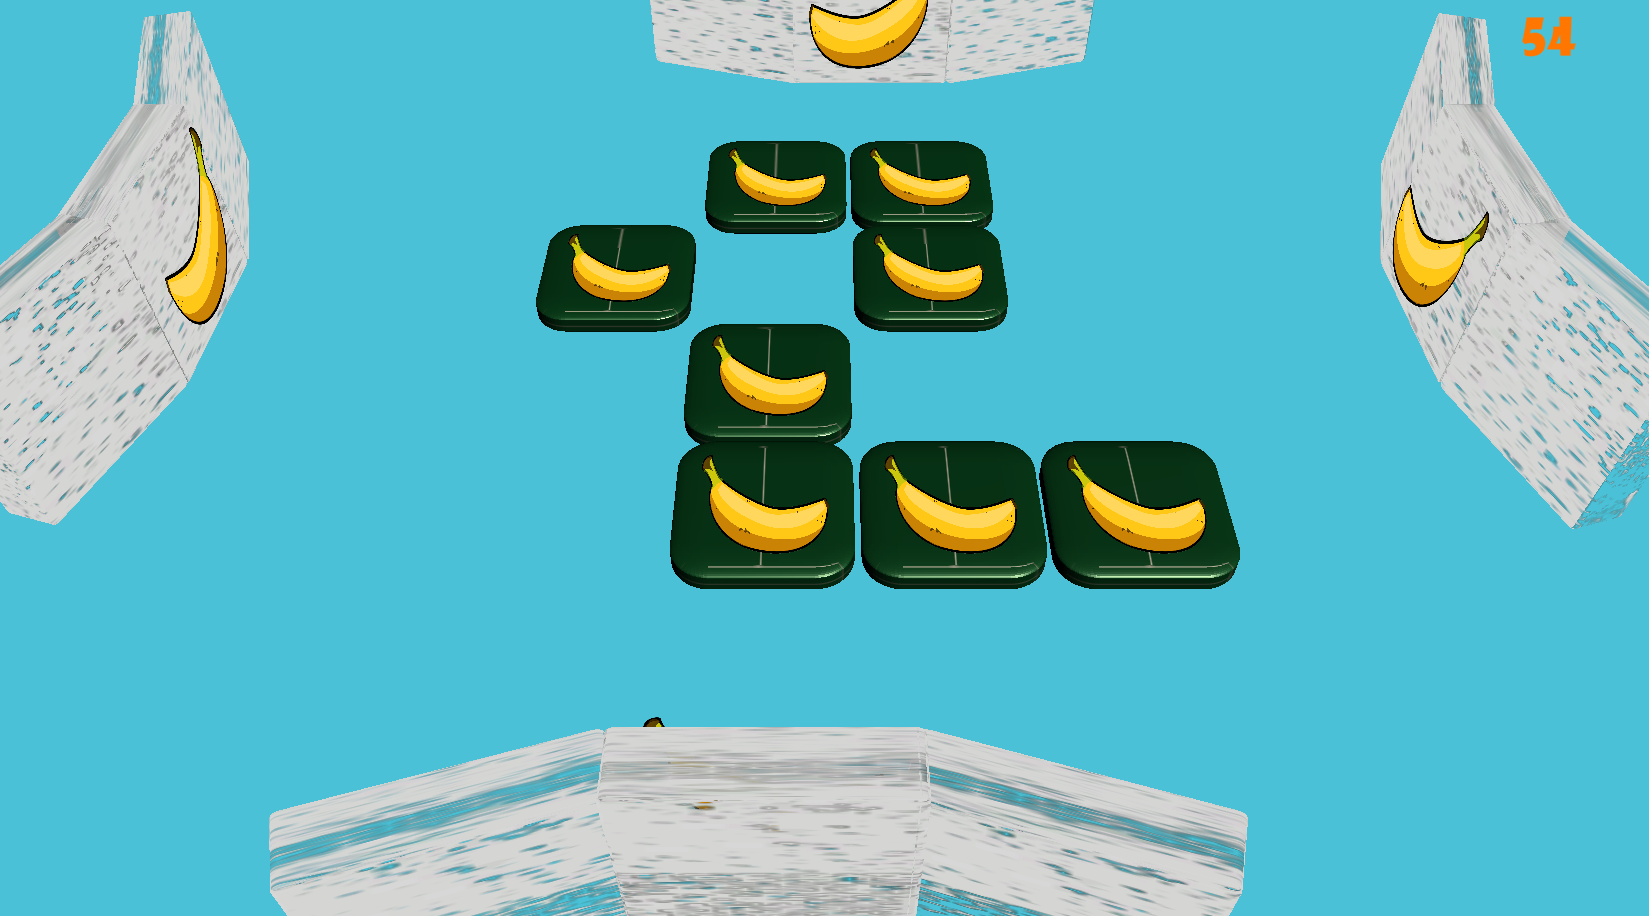
\includegraphics[width=0.9\textwidth]{perfectmatchpic.png}
	\end{center}
\end{column}
\end{columns}
\end{frame}

%%%%%%%%%%%%%%%%%% Slide %%%%%%%%%%%%%%%%%%
\begin{frame}{Probleme}
\begin{itemize}
 \item Multiplayer 
 	\begin{itemize}
 		\item Auch mit Framework aufwendig bis alle Details verstanden sind
 		\item Scripte an Synchronisation anpassen macht wenig Spaß
 		\item Testen schwierig/aufwendig, da Fehler oftmals erst nach Host/Client Wechsel, Rundenwechsel, etc. auftauchen
 	\end{itemize}
 \item Probuilder
 	\begin{itemize}
 		\item (Unity-)Koordinaten 
 		\item Snapping local/global
 	\end{itemize}
  \item Git
 	\begin{itemize}
 		\item Zeitaufwendig merge-conflicts auf Grund von Parameter Änderungen auf Objekten durchzugehen
 	\end{itemize}
  \item Blender zusammen mit Unity 
  \item Unity selbst!
\end{itemize}
	
\end{frame}

%%%%%%%%%%%%%%%%%% Slide %%%%%%%%%%%%%%%%%%
\begin{frame}{TuttiFrutti - Planung und Umsetzung}
\begin{itemize}
		\item überhaupt Stichpunkte explizit aufschreiben?
\end{itemize}
\begin{center}
		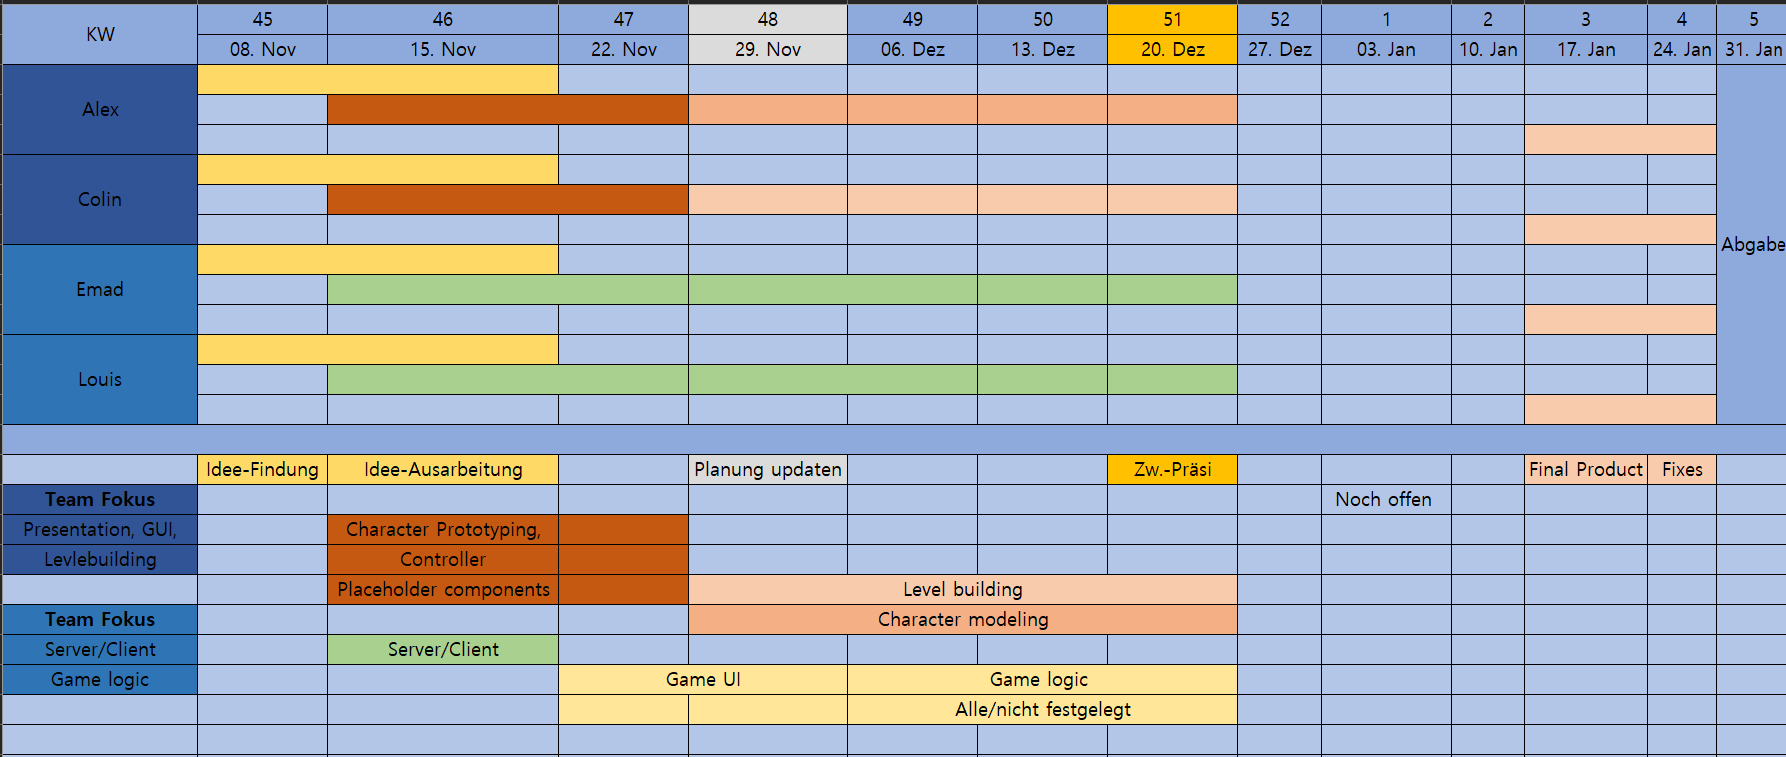
\includegraphics[width=1\textwidth]{ProjektPlanung_6times90.png}
\end{center}

\end{frame}

%%%%%%%%%%%%%%%%%% Slide %%%%%%%%%%%%%%%%%%
\begin{frame}{Ausblick}
\begin{itemize}
 		\item Tiefere Integration von (Steam)Multiplayer Komponenten
 			\begin{itemize}
 				\item (Voice-)Chat
 				\item (Steam-)Achievements
 			\end{itemize}
 		\item Seasons
 			\begin{itemize}
	 			\item Level + Modi Updates
	 			\item Where are the coins?
 			\end{itemize}
 		\item Globales player-ranking
 		\item Weitere Player-Moves, wie Dinge Werfen
\end{itemize}

\end{frame}

%%%%%%%%%%%%%%%%%% Slide %%%%%%%%%%%%%%%%%%
\begin{frame}{Live-Demo}

\begin{center}
	\Huge{\textcolor{OliveGreen}{Let´s play TuttiFrutti!}}
\end{center}

\end{frame}
%%%%%%%%%%%%%%% End of Slides %%%%%%%%%%%%%%%
\end{document}
